\documentclass{projectreport}
\usepackage{projectreportcommands}
\usepackage{lipsum}
\usepackage{graphicx}
\usepackage{listing}
\usepackage{tabularx}
\usepackage{cite}

\defstudentnameone{John Doe I}
\defstudentregnoone{1200XXXXX}
\defstudenttitleone{Mr.}

\defstudentnametwo{John Doe II}
\defstudentregnotwo{1200YYYYY}
\defstudenttitletwo{Mr.}

\defstudentnamethree{John Doe III}
\defstudentregnothree{1200ZZZZZ}
\defstudenttitlethree{Ms.}

\defprogramme{Computer Science and Engineering}

\defguide{John Doe}
\defguidedesignation{Senior Assistant Professor}
\defguideinstitution{Institution}
\defdegree{B. Tech Computer Science and Engineering}
\defsemester{May 2020}
\defschool{School of Computing}
\defpronouniwe{We} % I/We
\defpronounmeus{us} % me/us
\defstudyduration{2019 - 2020}

\title{Paper Title}
\date{18 November 2019}

\newcommand{\nomenclature}{
	\begin{center}
		\Large \textbf{NOMENCLATURE}\\
	\end{center}
	\begin{table}[h]
	\Large \textbf{English Symbols}\\
	\begin{tabular}{ll}
	$k_d$&Microbial decay coefficient\\
	$K_s$&Substrate concentration when growth rate is half of maximum\\
	Hz&Hertz\\
	\end{tabular}
	\end{table}
	\begin{table}[h]
	\Large \textbf{Greek Symbols}\\
	\begin{tabular}{ll}
	$\alpha$&Rate\\
	$\sigma(x)$&the standard deviation of x\\
	$\Sigma$&Summation\\
	\end{tabular}
	\end{table}
	\begin{table}[h]
	\Large \textbf{Miscellaneous Symbols}\\
	\begin{tabular}{ll}
	$|x|$&Absolute value of $x$\\
	\end{tabular}
	\end{table}
}

\begin{document}
	\pagenumbering{roman}
	\makereportfirstpage
	\bonafide
	\declaration
	\acknowledgement{\lipsum[1]}
	\newpage
	\tableofcontents
	\newpage
	\fakesection{List of Figures}
	\listoffigures
	\newpage
	\fakesection{List of Tables}
	\listoftables
	\newpage
	\nomenclature
	\newpage
	\reportabstract{
		This is some dummy abstract. \lipsum[2]
	}{Random, Keywords, for, report}
	\newpage
	\newpage
	\pagenumbering{arabic}
	\setcounter{page}{1}
	\chapter{Introduction}
		\setcounter{chapter}{1}
		\section{Some Intro Section}
		\lipsum[3]
		\section{Proposed Solution}
		\lipsum[4]
		\subsection{The Dataset}
		\lipsum[5]
	\chapter{Merits and Demerits of the Base Paper}
		\section{Existing Solution}
		\lipsum[6]
		\section{Merits}
		\lipsum[7]
		\section{Demerits}
		\lipsum[8]
	\begin{hyphenatedcode}
	\chapter{Source Code}
	\section{Sample Class}
	Purpose of the sample class is to show a sample python syntax. To add more keywords or words to emphasize, add them to line 78 and 80 in the file named miniprojectreport.cls\\Also, this\cite{7457930} is a dummy citation.\\
\begin{lstlisting}
# This is a sample code
class SampleClass:
    def __init__(self):
        self.x = 10	
\end{lstlisting}
	\end{hyphenatedcode}
	\newpage
	\chapter{Snapshots}
	\section{Sample Output screens}
	Add Snapshots of your output screen like Figure \ref{figureone}.
	\begin{figure}
		\centering
		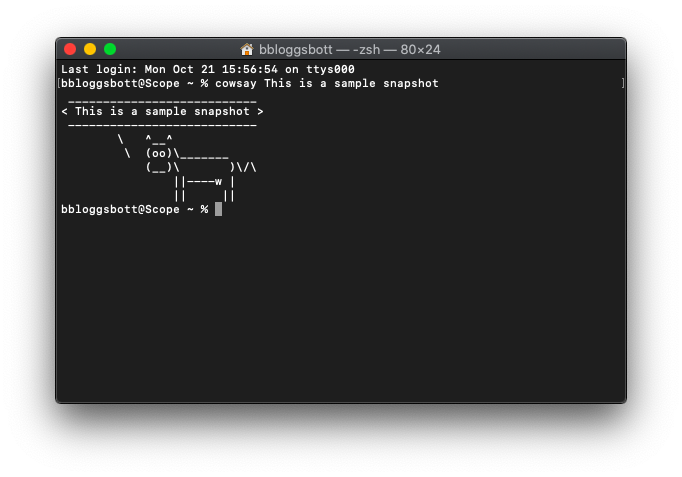
\includegraphics[width=\textwidth]{images/snapshot1}
		\caption{Sample Snapshot 1}
		\label{figureone}
	\end{figure}
	I'd suggest inverting color of terminal to save ink while printing like in Figure \ref{figure2}.
	\begin{figure}
		\centering
		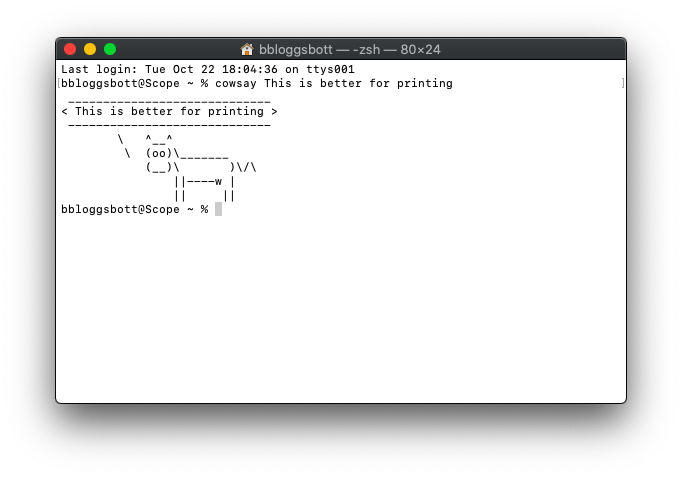
\includegraphics[width=\textwidth]{images/snapshot2}
		\caption{Sample Snapshot 2}
		\label{figure2}
	\end{figure}

	\chapter{Conclusion and Future Plans}
	\lipsum[9]\\

	\bibliography{projectreportbib}
	
	\bibliographystyle{ieeetr}
	
\end{document}
